%% LyX 2.2.3 created this file.  For more info, see http://www.lyx.org/.
%% Do not edit unless you really know what you are doing.
\documentclass[english]{article}
\usepackage[T1]{fontenc}
\usepackage[latin9]{inputenc}
\usepackage{geometry}
\geometry{verbose,tmargin=3cm,bmargin=3cm,lmargin=2cm,rmargin=2cm}
\usepackage{fancyhdr}
\pagestyle{fancy}
\usepackage{babel}
\usepackage{float}
\usepackage{endnotes}
\usepackage{graphicx}
\usepackage{setspace}
\usepackage{esint}
\usepackage[unicode=true,pdfusetitle,
 bookmarks=true,bookmarksnumbered=false,bookmarksopen=false,
 breaklinks=false,pdfborder={0 0 0},pdfborderstyle={},backref=false,colorlinks=false]
 {hyperref}

\makeatletter

%%%%%%%%%%%%%%%%%%%%%%%%%%%%%% LyX specific LaTeX commands.
\newcommand{\noun}[1]{\textsc{#1}}
%% Because html converters don't know tabularnewline
\providecommand{\tabularnewline}{\\}

%%%%%%%%%%%%%%%%%%%%%%%%%%%%%% Textclass specific LaTeX commands.
 \let\footnote=\endnote

\makeatother

\begin{document}
\begin{onehalfspace}

\title{CS282R Final Project: Interpretable deep RL based policies for Sepsis
treatment}
\end{onehalfspace}
\begin{onehalfspace}

\date{December 14th, 2017}
\end{onehalfspace}
\begin{onehalfspace}

\author{Camilo L. Fosco, Sebastien Baur - Harvard University\\
}
\end{onehalfspace}
\maketitle
\begin{onehalfspace}

\lhead{Camilo L. Fosco, Sebastien Baur, - CS282r}
\end{onehalfspace}

\section{Abstract }

\paragraph{According to www.cdc.gov, about 15\% of septic patients die in American
ICUs each year. This condition is severe, and treatments are both
expensive and challenging. Today, there is no consensus in the medical
world on how to treat septic patients, who all respond differently
to medications. The recent availability of public data for Sepsis
treatment, as well as the advances of deep learning and reinforcement
learning, allowed data-driven approaches to produce policies reducing
by more than 3\% the mortality rate. While the results are promising,
neural networks have the inherent drawback of being hard-to-understand
black boxes. The treatment policy obtained by these models can seem
obscure to physicians, while interpretability looks like an important
characteristic when it comes to saving lives. Recently, some work
proposed the ICNN architecture, a neural network that is convex with
respect to some of its inputs. In the context of deep RL applied to
the Sepsis problem, this property can be useful for several reasons:
the discrete representation of actions can be replaced by a richer
continuous representation, and the output of the Q network can be
concave and therefore has a unique maximum, which translates the idea
that there is an optimal dose to prescribe to the patient. This work
is our effort to improve previous work by making policies more interpretable
thanks to both the ICNN architecture and a different representation
of patients. }

\section{Introduction }

Sepsis is a severe condition, and treating it is challenging. It can
involve, among other: antibiotics to cure the infection, renal therapy
for patients having renal failures, mechanical ventilation to assist
patients having respiratory troubles, or prescription of medications
to correct hypovolemia. As described in Raghu et al \cite{raghu2017continuous},
here, we tackle the problem of prescribing the good doses of vasopressors
and intravenous fluids, which are particularly critical to the patient
survival (Waechter et al. \cite{waechter2014interaction}) As there
is not really any clear guideline on how these prescriptions should
be made, we propose to use a data-driven approach to this problem.
RL seems to be particularly suited to the task, as it involves taking
sequential decisions having potentially delayed consequences. While
recent advances in deep learning make neural networks powerful function
estimators, Mnih et al. only very recently successfully managed to
combine them with Q learning, giving birth to DQN. van Hasselt et
al., Wang et al. proposed improvements making it more stable, respectively
double DQN and dueling double DQN. This last version was used by Raghu
et al. to tackle the problem of prescribing vasopressors and intravenous
fluids. They also used sparse autoencoders to represent the health
states of the patients at a given time point, assuming that these
are Markovian. This improved the performance of their DQN algorithm.
However, it makes the obtained policy even less transparent.

This is why we proposed two main improvements to this approach: 
\begin{itemize}
\item Using variational autoencoders (VAE) (Kingma et al.) instead of sparse
autoencoders to represent the whole histories of the patient instead
of unique time steps. Encoding the whole histories instead of the
values at a given time point makes the Markov assumption more realistic.
We believe that using more information may improve the performance
of the obtained policies. VAE have two major advantages: they often
learn an interpretable latent representation, and they are generative
models. Generating new histories would make policy evaluation easier. 
\item Using the ICNN architecture Amos et al. for our Q network. It implies
that actions are continuous, which is a richer and more accurate representation
that discrete buckets. While it makes the problem a bit more complex
in terms of optimization, it is still quite easy because the Q network
is concave. It makes the obtained policy more interpretable, because
it translates the idea that the correct dose of medications to prescribe
is unimodal and has a unique maximum. It also allows the policy to
encode uncertainty, for example when it plateaus around some value;
conversely it can encode certainty, when the actual output is peaked
around a given dose. 
\end{itemize}

\section{Background and related work }

\subsection{Reinforcement learning }

The RL framework involves an agent interacting with its environment
at discrete time steps, trying to maximize the cumulative (or discounted)
reward that it reaps along the way. At each time step t, the world
is in a state $s_{t}$, and the agent can take an action $a_{t}$
from a given set of allowed actions A. This action allows it to transition
to the next state $s_{t+1}$, getting a reward $r_{t}$ during this
transition. The objective of the agent is to maximize the expected
sum of discounted rewards, $E[\sum_{t=1}^{T}\gamma^{t}r_{t}${]} if
there is given known time horizon T, or $\sum_{t=1}^{\infty}\gamma^{t}r_{t}$
if there is no time limit, where $\gamma$ is a discount factor between
0 and 1 that captures the trade-off of immediate vs. delayed rewards.
The optimal value function $Q^{*}(s,a)$ is the maximum expected discounted
reward after executing action a in state s, and then following the
optimal policy $\pi^{*}$, which consists in choosing actions greedily
on Q{*}. Q{*} verifies the Bellman optimality equation:
\[
Q^{*}(s,a)=E_{s'}[r+\gamma max_{a'}Q^{*}(s',a')]
\]

In the Sepsis problem, the states can naturally be the set of physiological,
lab, and demographic values that are attached to each patient at a
given time step. This representation is problematic for different
reasons: 
\begin{itemize}
\item It assumes that these states are Markovian. What happened to the patient
in the past is certainly relevant to its health state. We doubt that
using only these values at a given time point gives the physician
all the information it would need to make an informed decision.
\item Even though they are all the information we can have about the patient,
we believe that these quantities do not represent what the patient
actually is. We would rather consider them as partial observations
of a hidden state. 
\end{itemize}
We propose variational autoencoders as a solution to both these problems.

\subsection{Variational autoencoders }

Kingma et al. recently introduced a neural network architecture allowing
to perform variational inference in an efficient manner. This architecture
consists of two neural networks, the encoder that tries to predict
the latent variables \emph{z }from the input \emph{x}, and the decoder
that tries to reconstruct the input \emph{x} from the latent representation
\emph{z} (hence the name autoencoder). The output of both neural network
are stochastic. In practice it means that they have several deterministic
outputs, that consist in the parameters of a given distribution, for
example Gaussian. Then, using the \textquotedblleft reparameterization
trick\textquotedblright , i.e by introducing some noise as an additional
input, the output becomes stochastic. The concatenation of the two
neural networks can be trained end to end using backpropagation. The
objective function is: 
\[
L(x)=KL(q_{\psi}(z|x)\,||\,p(z))-E_{z\sim q_{\psi}(.|x)}[log(p_{\theta}(x|z))]
\]

Where the first RHS term is the KL divergence between the posterior
distribution $q_{\psi}(z|x)$ (the encoder, parametrized by $\psi$)
and the prior $p(z)$ which is usually a very simple distribution,
for example multivariate Gaussian. This terms forces the posterior
to be Gaussian, which, once trained, allows to sample new latent codes
to generate new data points. The second term is the negative log likelihood.
It forces the neural network to have accurate reconstructions of the
inputs. $p_{\theta}(x|z)$ is the decoder neural network, parametrized
by $\theta$. The loss L(x) is bound on the log evidence $log(p_{\theta}(x))$
(Blei et al.) 

One key observation that has been made by training these models, is
that the latent representation they learn naturally arranges in meaningful
way. For example, the MNIST digits get clustered together in the latent
space (Figure \ref{fig:The-2D-latent-space-VAE}), while no information
allows the model to distinguish classes. When trained on pictures
of faces (Hou et al.), the latent representation naturally encodes
the color of the hair, whether the person is smiling or not, wearing
glasses or not, the angle of the head, etc. On more complex datasets
such as molecules, the latent representation will include information
such as the function of the molecules or physical properties. (Gomez
Bombarelli) 

\begin{figure}[H]
\centering{}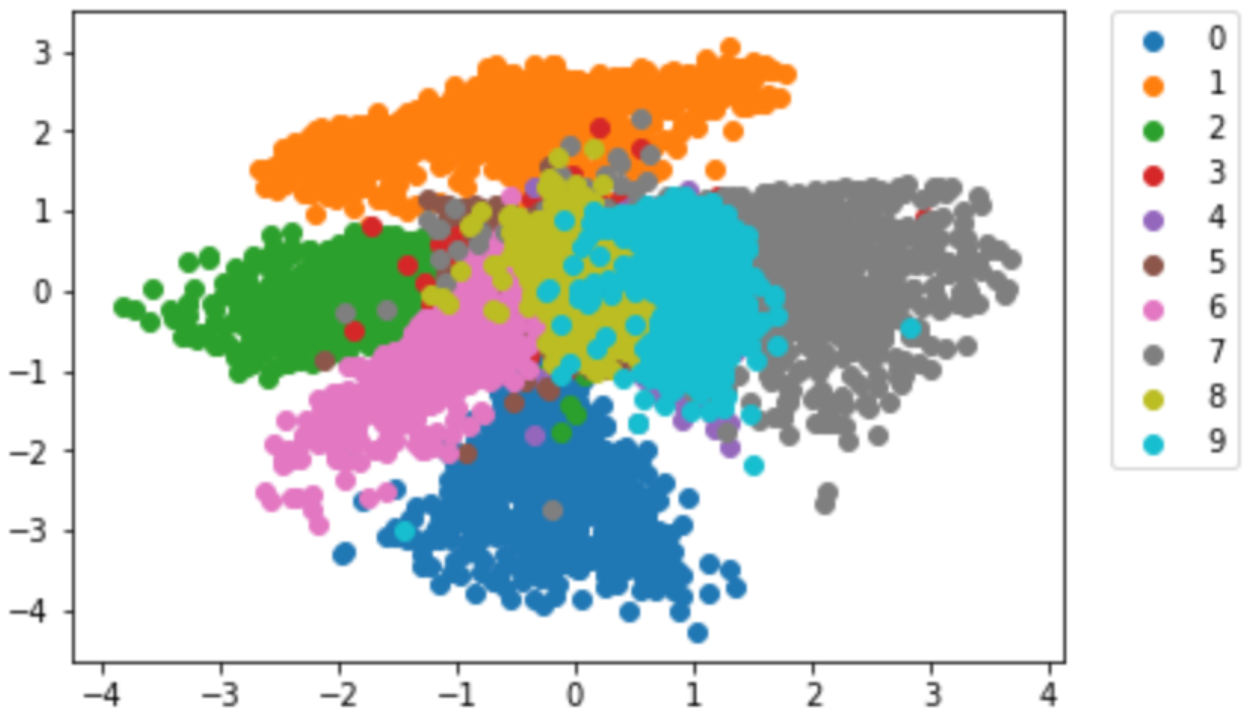
\includegraphics[width=0.4\paperwidth]{figure/fig1.PNG}\caption{\emph{The 2D latent space of a VAE trained on the MNIST dataset. The
latent space naturally arranges by clustering the digits together.
Note that the digits that can be similarly written, share common frontiers.
Ex: 9 with 7 and 9 with 8\label{fig:The-2D-latent-space-VAE}}}
\end{figure}

In the case of the Sepsis problem, we propose using VAEs to encode
the histories of the patients. It means that whole histories would
be encoded by a latent code \emph{z }having a simple prior \emph{p(z)}.
One of the inputs of our Q network would be this latent representation.
By encoding whole histories instead of unique time points, the trained
model can then sample new whole histories, or predict the end of a
given history, instead of sampling values at a given time point. It
therefore makes it possible to generate episodes with a chosen policy,
and estimate the mortality associated with this policy. Our model
would actually be a conditional VAE (CVAE) (Sohn et al.), which differs
from a vanilla VAE in that both the encoder and the decoder have an
additional input, their outputs being conditional on this. Consequently,
it gives some control on what is generated. In our case, it would
allow to see the impact of a given action on the health state of the
patient.

\begin{figure}[H]
\begin{centering}
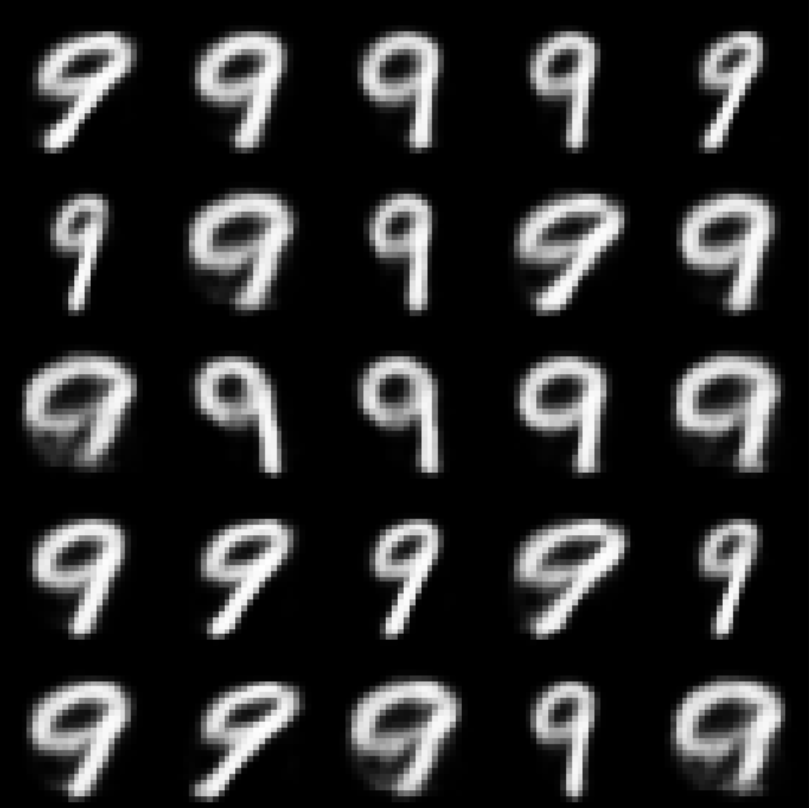
\includegraphics[width=0.4\paperwidth]{figure/fig2.PNG}\caption{\emph{Generation conditioned on the digit 9. Contrary to Figure 1,
the latent code no longer encodes anything relative to what the digit
is, but rather to how the digits looks. }}
\par\end{centering}
\end{figure}

\subsection{Input Convex Neural Networks}

The Input Convex Neural Network (ICNN) is an architecture proposed
by Amos et al. that makes a neural network convex with regard to some
of its inputs.

\begin{figure}[H]
\centering{}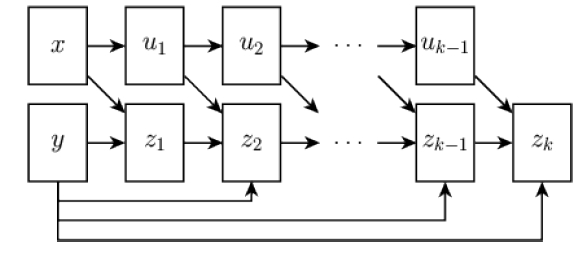
\includegraphics[width=0.4\paperwidth]{figure/fig3.PNG}\caption{\emph{A neural network convex w.r.t }y\emph{.}}
\end{figure}

The network is convex if its layers verify:
\begin{center}
\includegraphics[width=0.3\paperwidth]{\string"figure/ICNN formulas\string".png}
\par\end{center}

Where $\circ$ is the element-wise product, and $\tilde{g}_{i},\,g_{i}$
are non-decreasing convex nonlinear functions. As we want the neural
network to be concave, we take $-z_{k}$ instead of $z_{k}$.

\begin{figure}[H]
\centering{}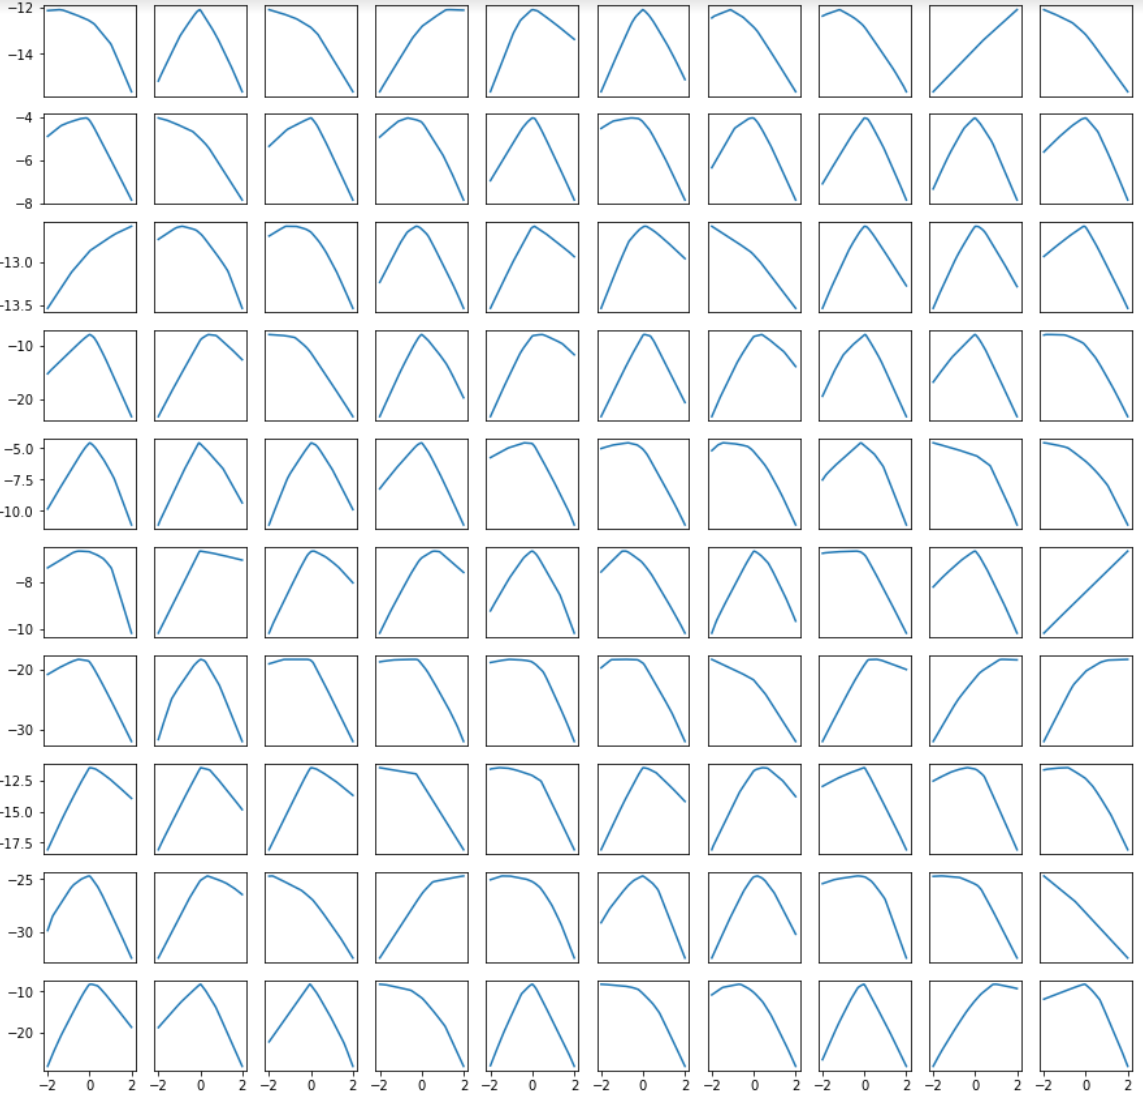
\includegraphics[width=0.6\paperwidth]{figure/fig4.PNG}\caption{\emph{Output of the ICNN with randomly initialized weights. The x
axis of each graph is one of the inputs for which the model is concave.
The other one is fixed, and is the same in each graph. Each graph
represents a different state. One can notice that the output can be
more or less peaked. If the policy is chosen to be proportional to
Q then plateaus correspond to uncertainty about the optimal dose,
and peaks correspond to certainty. The output can be monotonic if
the optimal dose to prescribe is either the maximal or minimal possible
dose.}}
\end{figure}

\subsection{Policy evaluation }

The challenge of accurate policy evaluation is an active area of research
in Reinforcement Learning, and off-policy evaluation - evaluating
the strategy when it is too costly to test it on the real world situation
it is designed for - is one of the main problems currently being analyzed.
The central idea of this field is to use data generated from a certain
policy to estimate the value of a new one. There is a large amount
of work in that area: methods such as importance sampling/weighting
(Doina Precup, 2000), Doubly Robust Estimator (REF) and the MAGIC
estimator (REF) have been shown to produce accurate estimations and
possess beneficial properties, from unbiased, consistent estimations
to lower variance in values. In this project, we mainly focused on
the Doubly Robust (DR) and Weighted Doubly Robust (WDR) estimators. 

\subsubsection{Importance sampling }

Importance sampling is typically presented as a method for reducing
the variance of the estimate of an expectation by carefully choosing
a sampling distribution (Rubinstein 1981). The idea is to choose a
distribution $q(x)$ to reduce the variance of the estimate of $\int f(x)p(x)dx$,
and can be viewed as trying to approximate $\int f(x)\frac{p(x)}{q(x)}q(x)$
with samples drawn from $q(x)$. As long as $p(x)$ and $q(x)$ have
the same support, this estimation is unbiased. In our setting, we
can consider that every policy induces a probability distribution
over histories. We want to estimate the expected return of an evaluation
policy given the history probability induced by a behavior policy.
importance sampling allows us to handle the mismatch between samples
generated from these two different policies. The statistical approach
to importance sampling is to find an appropriate $q(x)$ to reduce
variance given an estimator - in our case, we have a fixed q stemming
from the behavior policy, and we are trying to determine the value
of the estimator itself given our data. A variant of IS, Weighted
importance sampling, weights each sample by the sum of $\frac{p(x)}{q(x)}$
for the dataset. This produces a biased estimator, but a faster, consistent
and more stable one than the high-variance IS. These importance sampling
estimator is a key concept underlying both estimators utilized in
this work.

\subsubsection{Doubly Robust Estimator}

This estimator aims to provide a solid approximation of a given policy
by leveraging two techniques that are known two work in two different
situations. One approach to OPE is to try to fit an MDP to the dataset,
and evaluate the target policy on the resulting model. This has usually
low variance, but is dependent on a correct modeling of the transitions
and rewards of the underlying process. The other approach is the IS
method discussed previously - unbiased and independent of characteristics
of the underlying model, but with high variance and dependent on the
similarity between the evaluation and behavior policies. The novelty
of DR is to combine these approaches to benefit from both worlds:
the resulting estimator designed by Jiang and Li attains high accuracy
while remaining unbiased. The latest formulation for this estimator
is as follows:

\[
DR(D):=\sum_{i=1}^{n}\sum_{t=0}^{\infty}\gamma^{t}\omega_{t}^{i}R_{t}^{H}-\sum_{i=1}^{n}\sum_{t=0}^{\infty}\gamma^{t}\left(\omega_{t}^{i}\hat{q}^{\pi_{e}}(S_{t}^{H_{i}},A_{t}^{H_{i}})-\omega_{t-1}\hat{v}^{\pi_{e}}(S_{t}^{H_{i}})\right)
\]

Where $\omega_{t}=\rho_{t}^{i}/n$, n being the amount of histories
(or trajectories), $\rho_{t}^{i}$ being the importance weight for
the first t steps of trajectory i (probability of first t steps of
history H under policy $\pi_{e}$), S and A are the states and actions
of a history, $\gamma$ is the discount factor, and $\hat{q},\hat{v}$
are estimations of the Q and V functions of the underlying MDP. As
can be understood from the equation, both OPE approaches described
are present here, as the importance weights and the q,v estimations
influence the value of the final estimator.

\subsubsection{Weighted Doubly Robust Estimator}

The weighted doubly robust estimator is different to DR in that it
incorporates the concept of Weighted Importance sampling . It extends
the DR concept by weighting the $\omega_{t}^{i}$ coefficients such
that $\omega_{t}^{i}=\rho_{t}^{i}/\sum_{j=1}^{n}\rho_{t}^{j}$. WDR
is not an unbiased estimator, but as mentioned by the authors, the
unbiasedness of these estimators is not paramount, as one of the advantages
of unbiased methods, computing confidence bounds on $v(\pi_{e})$,
only comes into play when the volume of data is high, which is impractical
in real world situations. WDR produces better estimates of $v(\pi_{e})$
when measured through MSE, which is ultimately the objective, as it
gets closer to the balance in bias-variance trade-off that approaches
optimality on the estimation.\\

In the Sepsis problem, the situation is appropriate for evaluating
the policy with these techniques, as we possess a large amount of
data acquired with one or multiple policies different than the one
we want to evaluate. The challenge lies in identifying the correct
behavior policy. We particularly investigated DR and WDR. It is important
to notice that in our setting, both states and actions are continuous,
and as such, the estimators must be applied having this in mind.

\subsection{Deep RL for the Sepsis problem }

The recent advances of deep RL, and more specifically dueling double
DQN (van Hasselt et al., Wang et al., Mnih et al., Schaul et al.),
were used by Raghu et al. to learn policies on the Sepsis dataset.
The states were either the 50 demographics, vitals, lab values of
the MIMIC dataset (see part \textquoteleft dataset\textquoteright ),
or the encoded version of these. The action space was quantized so
that each medication dose fits in one of the five bins, leading to
a total of 25 possible actions. Obtained policies were evaluated to
reduce by 3.6\% the mortality rate, which is very encouraging.

However, this approach has the downfall of being difficult to interpret
and analyze - the policies obtained cannot be evaluated in a very
rigorous manner, as their analysis depends highly on the behavior
of the clinician's policy, and approximating that policy with the
MIMIC dataset is no trivial task. Besides, the best model used encoded
vitals/demographics/lab values, which makes the behavior of the network
harder to interpret. There is no clear way of understanding the reasoning
of the approach, which is critical in a medical environment, and the
distribution of actions generated by the network may not adhere to
certain critical concepts known by clinicians. 

This is the motivation for the VAE idea: being a action-conditioned
generative model, our VAE would allow us to generate new histories
to evaluate policies. As the latent representation it learns naturally
arranges in a meaningful way, our state representation may be more
interpretable for physicians. As it would allow to encode full histories,
the Markovian assumption is no longer a problem. 

Discussions with physicians led to the hypothesis that there must
be one optimal dose of medication to prescribe to the patient - this
dose can be 0. Indeed, it seems unlikely that two extremely different
doses may have similar beneficial effects. We therefore suppose that
the optimal policy should be unimodal. This is motivates the use of
the ICNN for our Q-network: it makes it concave, and therefore has
a unique maximum on the interval of possible actions. 

\subsection{Dataset}

We worked with the MIMIC database (ref). As preprocessing steps, we: 
\begin{itemize}
\item Dropped all patients having unrealistic values in any column (negative
values or values well beyond ranges of acceptable values)
\item Logged exponentially distributed quantities. If they could be zero,
we first added the minimum of the dataset.
\item Standard scaled all numerical quantities (operation that was performed
after the log for the quantities that were logged) 
\end{itemize}
The features are all the columns except those that are action-related
(fluids or vasopressors). \textquotedblleft Binary actions\textquotedblright{}
(mechanical ventilation, sedation, renal therapy) were included in
the state space. In total, it represents 50 demographics, vitals,
and lab values. 

\section{Development and Results}

\subsection{The VAE Approach}

Our VAE is trained to reconstruct full histories h. It is conditioned
on actions a. 

\begin{figure}[H]
\begin{centering}
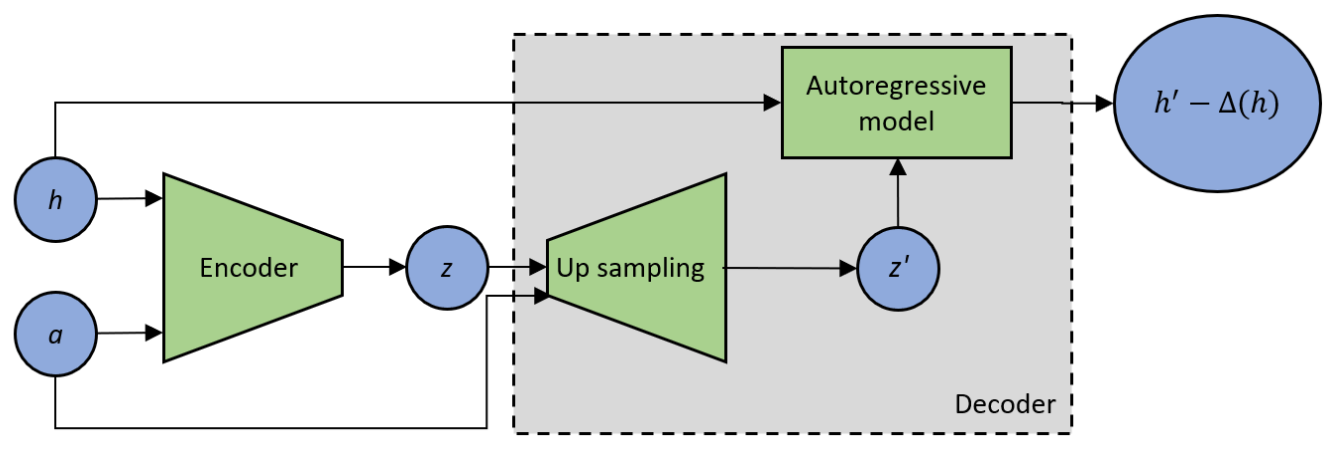
\includegraphics[width=0.6\paperwidth]{figure/fig5.PNG}\caption{\emph{Architecture of the VAE. The histories h are encoded in a latent
space. The latent representation z, comprises the states we use as
inputs of our DQN (instead of the initial 50 features). The decoder
first up-samples the latent code to make it the same dimension as
the history, and concatenates them on the channel axis. The obtained
array is passed to an autoregressive model that predicts the difference
between the t-th and the t+1-th time step from the t first time steps.}}
\par\end{centering}
\end{figure}

The loss is constructed as the MSE between true and generated histories,
and the KL divergence between the latent code and a multivariate standard
Gaussian: 
\[
L(h,h')=(h-h')^{2}+KL(q_{\psi}(z|h)\,||\,N(0,I_{d}))
\]

Where \emph{d }is the dimension of the latent space, and $q_{\psi}(z|h)$
is the output distribution of the encoder. As in Kingma et al., we
used a Gaussian distribution. In practice, the encoder has two outputs:
the parameters $\mu_{\psi}(h),\,\sigma_{\psi}(h)$ of the Gaussian
distribution. The reparameterization trick allows us to have $z|h\sim N(\mu_{\psi}(h),\sigma_{\psi}(h))$.

The encoder is a convolutional neural network. As the inputs don\textquoteright t
have the same length (patients stays have different durations), they
were padded with 0. We realized a bit late that it is not sensible
because most of the variables are continuous rather than binary. Some
possible fixes may be: 
\begin{itemize}
\item - Grouping histories by length during training 
\item Padding and masking the loss corresponding to the appended zeros 
\item Using a recurrent neural network as the encoder 
\item Using layers that have a known fixed size whatever the input dimension
is, for example max pooling over time. 
\end{itemize}
Unfortunately, we didn\textquoteright t have time to explore these
different options, which are necessary steps to having a working model.

The decoder is an autoregressive model. It was trained to predict
$h-\Delta h$ from \emph{z} and \emph{a}, where $\Delta h$ is a shifted
version of the history (its t-th component is the value of the t-1-th
component of h). This way, it learns to predict relative perturbations
rather than absolute values. We hope that learning perturbations will
help to generalize better. When generating a new history, it does
so sequentially, one step at a time. 

At first, we used an LSTM (Hochreiter et al) as our decoder architecture,
but it was too powerful - it didn\textquoteright t use the latent
code z at all during decoding (the output was constant with regard
to the latent code). Consequently, we tried less powerful stacks of
causal dilated convolutions (van den Oord), with varying receptive
field sizes. However, the model didn\textquoteright t use the latent
information anyway, even with very small receptive fields. 

It is still unclear to us why the VAE didn\textquoteright t use the
latent code during training. A discussion with Yoon Kim from the Harvard
NLP group made us conclude that there is a problem on how we perform
inference on the latent representation. Our latent representation
may not be adapted to the temporal structure of our inputs, for several
reasons: 
\begin{itemize}
\item The encoder is convolutional and the inputs are padded with zeros,
which means that extra meaningless information is encoded in the latent
representation. The shorter the history, the more the latent code
contains meaningless information. 
\item In the decoder, we up-sample this latent code before concatenating
it to the history (on channel axis) and passing it to the autoregressive
model. This is not really sensible since the history has a temporal
structure and the latent code does not. We believe that it would be
more sound to either not upsample the code at all - and rather repeat
it at each time step, as is commonly done in NLP - or have a latent
code per time step. Our time series being multidimensional, it may
be wiser to use a latent code per time step. In that case, the decoder
should perform inference on the code as well. 
\end{itemize}
Variational autoencoders had recently some success on temporal-structured
data. Using a model more like the one described in Chung et al., or
Krishnan et al., or Fabius et al. may lead to better results. These
models all use RNN for both the encoder and the decoder. The latent
code is either global (one for the whole sequence), or local (one
for each time step). In the second case, the decoder performs inference
on the latent code as well. This is something we would like to investigate
further in the future. 

In conclusion, the VAE approach was not fruitful. We think it is still
worth mentioning it because it could lead to interesting developments
in the future. As we could use only the vitals/lab values/demographics
as inputs of our Q network, we didn\textquoteright t investigate further
this path, and focused on the Deep Q Learning part of the project. 

\subsection{Deep Q Learning with ICNN }

We started by implementing our own DQN and ICNN using PyTorch. At
the time, we were working on the Sepsis problem. As we will soon explain,
we met problems we initially couldn\textquoteright t find the cause
of, so we decided to tackle a simpler problem. That\textquoteright s
why we designed the \textquotedblleft moving particle\textquotedblright{}
problem, described in one of the next paragraphs. We also applied
the network to a modified version of MountainCarContinuous, from OpenAI.
The policies obtained here were good but not ideal, so we decided
to compare our ICNN to the original implementation. We therefore created
a Tensorflow model adapted from the ICNN of LocusLab (github), the
original implementation that came out with the paper. We managed to
get interesting policies with this method. Here are some hyperparameters
we used, independently of the problem. 

\begin{table}[H]
\begin{centering}
\begin{tabular}{|c|c|}
\hline 
Parameters & Values\tabularnewline
\hline 
\hline 
Gamma & 0.99\tabularnewline
\hline 
Update Frequency & 100 or 200 steps if updated periodically, $\tau=10^{-2}$ or $10^{-3}$
if updated after each batch\tabularnewline
\hline 
Hidden dimension & 20 to 100 (closer to 20 for simpler problems, to 100 for Sepsis problem)\tabularnewline
\hline 
Number of layers & 2 to 3\tabularnewline
\hline 
Optimization algorith to find the maximal action & RProp, max 8-10 steps (PyTorch) / Adam, max 8-10 steps (Tensorflow) \tabularnewline
\hline 
Learning Rate & 1e-4, 1e-3 or 1e-2\tabularnewline
\hline 
Batch size & 32, 64, or 256\tabularnewline
\hline 
Prioritized Experience Replay Parameters & Default $\alpha$=0.6, $\epsilon=10^{-2}$, and starting at 0.9and
annealing linearly to 1 in 105batches\tabularnewline
\hline 
RMIN, RMAX, intermediate rewards & -15, 15, 0 for Sepsis problem Different schemes for the two other
problems \tabularnewline
\hline 
Nonlinearities & LeakyReLU(0.01), Softplus, or ReLU\tabularnewline
\hline 
\end{tabular}\caption{Range of hyperparameters used.}
\par\end{centering}
\end{table}

It is interesting to remark that RProp was the fastest algorithm to
find the maximum of Q(s, .) (tested empirically against all the other
optimization algorithms proposed in PyTorch). The Tensorflow implementation
used Adam, and we didn\textquoteright t change it. The weights of
the target network were updated either periodically, or after each
batch. In the 2nd case, we have:
\[
\theta_{i+1}^{-}\leftarrow(1-\tau)\theta_{i}^{-}+\tau\theta_{i+1}
\]
where $\tau$ is either $10^{-2}$ or $10^{-3}$ . This choice had
no significant impact on the training process.

\subsubsection{Sepsis problem }

Trying to train our Q network, we met mainly two related problems.
Even though we use double DQN, both the target and the main Q networks
tends to become very quickly overconfident after a few steps of training.
Besides, the output of the Q network (both target and main) is most
of the time linear rather than U-shaped, which is not really what
we expect. 

In most of our experiments, we observed that Q tends to become overconfident
very quickly, and even tends to diverge. The first solution we tried
was to add a sigmoid nonlinearity at the output, scaled to the range
$[R_{MIN},R_{MAX}]$. It makes the outputs non-concave, but still
very easy to optimize as a nondecreasing function of a concave function.
In terms of expressiveness, it is very similar or even better. It
allows to translate uncertainty, and the output is still unimodal.
It clips the values and therefore removes the explosion problem.

\begin{figure}[H]
\centering{}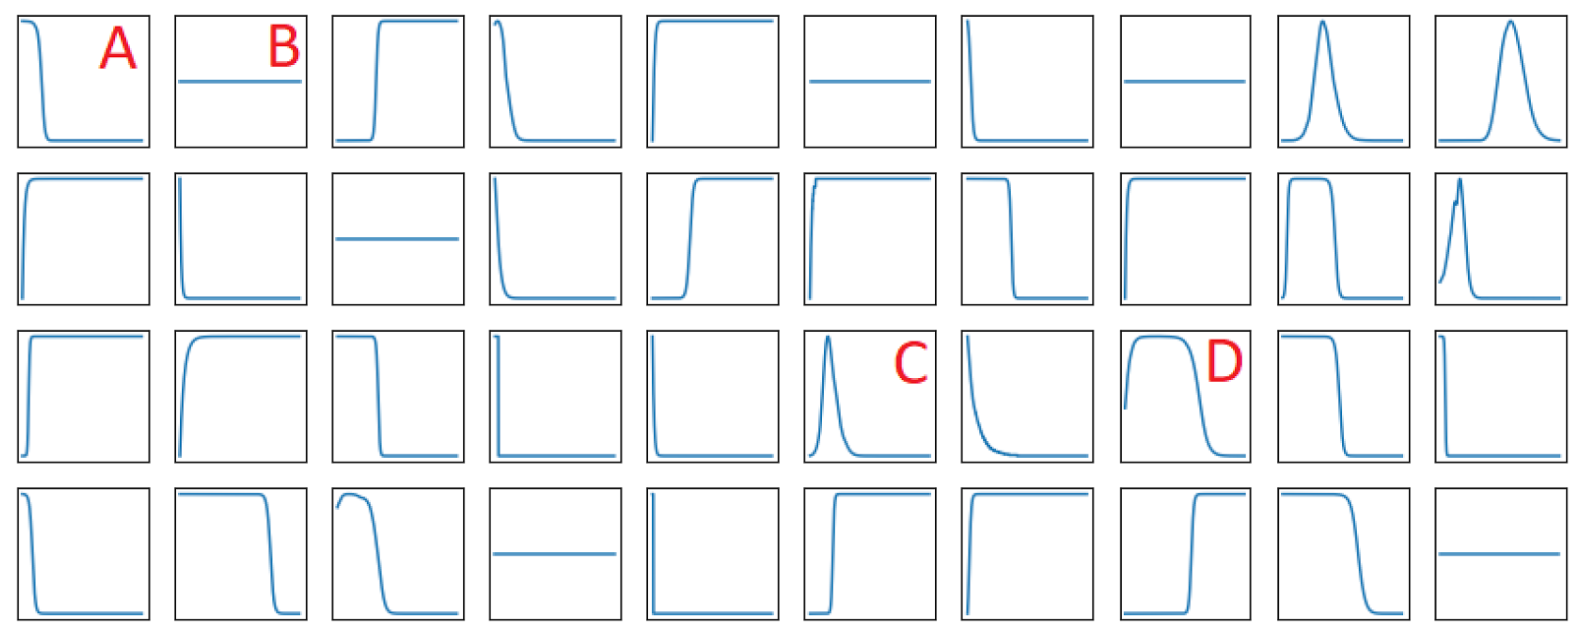
\includegraphics[width=0.6\paperwidth]{figure/fig6.PNG}\caption{\emph{Output of the model with an additional sigmoid layer, with randomly
initialized weights. The different possible shapes are still very
interpretable. In A, the model is quite certain that nothing should
be given to the patient, in B it has no idea, in C and D it should
give about the same quantity, but in D it is not very accurate.}}
\end{figure}

However, it raises a new problem: saturation at RMAX, making the problem
very hard to optimize (vanishing gradients). We tried two things to
solve the saturation problem: 
\begin{itemize}
\item We added batch normalization layers, that temper the vanishing gradient
problem.
\item We first logit the prediction and the target before computing the
MSE.
\end{itemize}
None of these two approaches worked, we therefore got rid of the sigmoid
output. 

Instead, we clipped the targets to the range $[R_{MIN},R_{MAX}]$,
and added to the loss a term penalizing the predictions outside of
the range $[R_{MIN},R_{MAX}]$. The loss therefore became:
\[
(Q_{\theta}(s,a)-r-\gamma Q_{\theta^{-}}(s',argmax_{a'}Q_{\theta}(s',a')))^{2}+c\cdot(Q_{\theta}(s,a)-R_{MAX})^{2}I_{Q_{\theta}(s,a)>R_{MAX}}+c\cdot(Q_{\theta}(s,a)-R_{MIN})^{2}I_{Q_{\theta}(s,a)<R_{MIN}}
\]

Where $Q_{\theta}$ is the main network, and $Q_{\theta^{-}}$ is
the target network. $I_{A}$ is the indicator of the condition A,
which is 1 if A is true, and 0 otherwise.

With \emph{c} high enough, this trick removed the divergence problem.
However, the network stays overconfident and we observed that the
output saturated at $R_{MAX}$. To understand this, note that predicting
always $R_{MAX}$ yields a small loss. Indeed, for survival terminal
transitions, that represent about 8\% of the dataset, the loss will
be 0. For non-terminal transitions, that represent about 90\% of the
dataset, its loss will be $(1-\gamma)^{2}R_{MAX}^{2}$, which is quite
small too, as we have $1-\gamma=0.01$. Only for death terminal transitions,
the loss is very important: $(R_{MAX}-R_{MIN})^{2}$. However, these
transitions represent only about 2\% of the dataset. As there is initially
no priority on the transitions, the model is presented with 98\% of
transitions for which predicting RMAX will lead to small error. It
therefore very quickly saturates. 

To alleviate this problem, we tried several things: 
\begin{itemize}
\item First, we prioritized terminal transitions before any training. This
did not help, we continued to observe Q saturation at $R_{MAX}$.
An idea that we have not explored may be to prioritize only death
terminal transitions. 
\item We also tried to start with a buffer containing equal proportions
of terminal and nonterminal. Then, new batches of data were added
as training went on. Unfortunately, it led to the same result. 
\item We also tried to reduce the learning rate from $10^{-2}$ to $10^{-3}$
and $10^{-4}$ and clipped the gradients, while increasing the PER
prioritization parameter $\alpha$. The objective was to force PER
to show the neural network many death terminal transitions before
it starts being over confident. While it helped alleviating the problem,
the final result was again the same: saturation of the neural network
at $R_{MAX}$. 
\item Clipping the targets to the range $Q_{\theta}-1,Q_{\theta}+1$ also
helped to reduce the speed at which the Q networks becomes overconfident,
but it leads to the same final result.
\end{itemize}
\textbf{\small{}Linear outputs situation: }We observed that, during
training, the action maximizing Q was always one of the four extreme
actions (as the actions are 2 dimensional, there are 4 extreme actions).
This suggested that the output of the neural network was always linear,
and not U-shaped. As \textquotedblleft doing nothing\textquotedblright{}
is the most chosen action in the dataset, it is not very surprising:
the policy of the physician could often be represented as a linear
decreasing function of a. We, however, expected the neural network
to learn U-shaped curves. We first verified in several settings of
the hyperparameters whether the output of randomly initialized neural
networks tended to be rather monotonic or U-shaped. This property
seems to be strongly dependent on the number of layers, the dimensions
of hidden layers, and the scale of the distribution of the initial
random weights. We couldn\textquoteright t find a proper way to always
start with U curves. We tried to test the ability of the neural network
to learn U-shaped concave function. For this, we designed a supervised
learning problem, where the inputs were $a_{1},a_{2},s$, and the
neural network tries to learn $-a_{1}^{2}-a_{2}^{2}+cos(10s)$. The
model was indeed able to learn this function, but was still producing
monotonic curves on Sepsis. To rule out the possibility of the ICNN
just not being adapted to the Sepsis dataset, we constructed two simpler
problems to observe the behavior of the network with more detail and
increased interpretability. 

\subsubsection{Moving particle problem }

\noun{Setup:} We first constructed a 2-dimensional motion problem,
which consists of a particle that has to reach a blue zone delimited
by a circle. The agent moves in the square $[-1,1]^{2}$, controlled
by acceleration (the actions are $a_{x},a_{y}$ and are continuous,
in the range {[}-1,1{]}). Its speed is also bounded by {[}-1,1{]}
on both x and y axis. When hitting a wall, the particle is elastically
reflected. The state space is 4D (position and speed), and the action
space 2D. The particle gets reward for reaching the disk of radius
0.5, centered at 0. Touching the circle leads to the end of the episode,
with reward 1.

\begin{figure}[H]
\begin{centering}
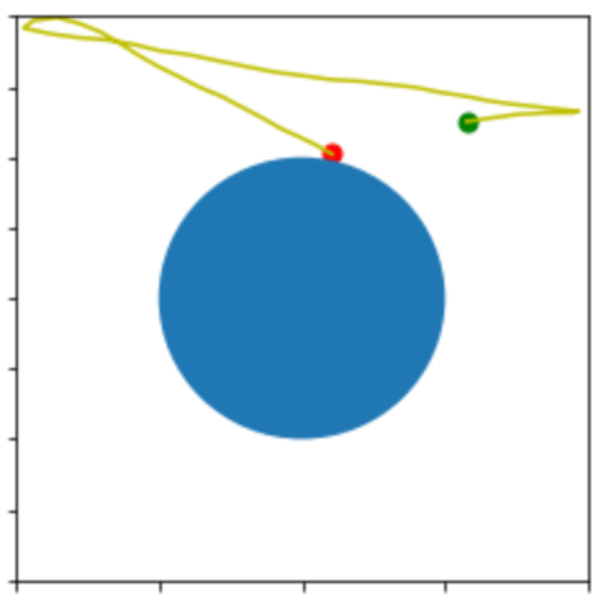
\includegraphics[width=0.5\paperwidth]{figure/fig7.PNG}\caption{\emph{Random trajectory of a particle, starting at the green dot and
finishing at the red dot.}}
\par\end{centering}
\end{figure}

To simulate the experience replay situation we were having with the
Sepsis case, we generated a few thousands episodes randomly before
training, and filled the PER buffer with these.\\

\noun{Discussion:} On this very simple problem, we still observed
that our Q network outputs were linear. It made the particle travel
around in half-circles, learning nothing useful. It seemed not to
take the rewards into consideration at all. As rewards were very sparse
(just as in the Sepsis problem), we kicked off the debugging process
by modifying the reward scheme to see if it could help the agent learn
a sensible policy. We tried two things: 
\begin{itemize}
\item We added a penalty based on the distance to the disk. This should
have forced the agent to go to the disk as fast as possible. Unfortunately,
it has absolutely no impact at all on the learned policy. 
\item We penalized extreme actions by adding a penalty on the square of
the acceleration. Again, we obtained linear outputs, the extreme action
just being shrinked towards 0. 
\end{itemize}
\begin{figure}[H]
\begin{centering}
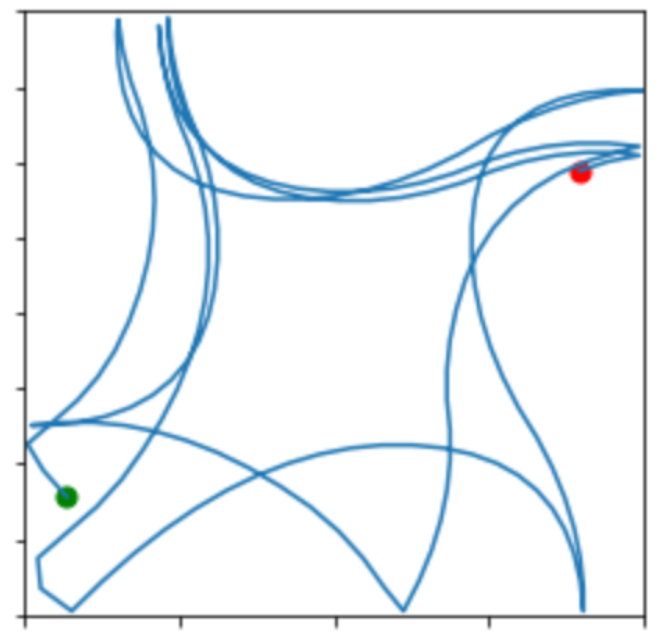
\includegraphics[width=0.5\paperwidth]{figure/fig8.PNG}\caption{\emph{Learned policy on the particle problem. The episode was not
stopped when reaching the disc to observe the agent's behavior. As
can be seen, the particle is always accelerating at the minimum or
maximum possible value, and thus its position takes the form of quadratic
curves.}}
\par\end{centering}
\end{figure}

As this problem did not give us further intuition on the problems
of the ICNN, we tried to observe its behavior on another problem.

\subsubsection{Mountain Car problem }

\noun{Setup:} We used the open source Gym from OpenAI, and more specifically
the problem MoutainCarContinuous depicted below.

\begin{figure}[H]
\begin{centering}
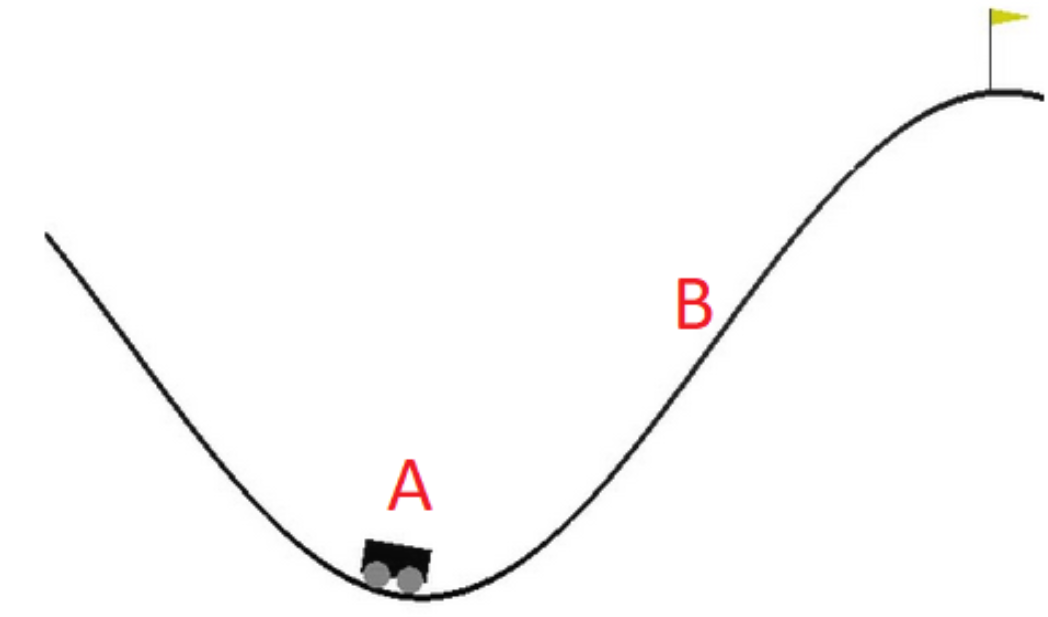
\includegraphics[width=0.5\paperwidth]{figure/fig9.PNG}\caption{\emph{Mountain Car Continuous. The starting point is in A. The agent
gets a positive reward if it reaches the flag. If it just accelerates
blindly, it reaches B, and then the gravity compensates its acceleration,
and it falls back to A. On the original environment, the agent gets
a negative reward at each time-step that is equal to the square of
its current acceleration (action).\label{fig:Mountain-Car-Continuous.}}}
\par\end{centering}
\end{figure}

As there is a negative reward on the square of the acceleration, the
optimal strategy consists in using gravity to reach the flag, by increasingly
oscillating around the starting position. The state space is the position
(1 dimensional value, in the range {[}-1.2, 0.6{]}) and the car velocity
(1 dimensional value in the range {[}-0.07, 0.07{]}). The action space
is one dimensional: it is just the positive or negative value of the
acceleration of the car. Acceleration is in the range {[}-1,1{]}.
The reward for reaching the flag is 100, and as was mentioned, there
is a penalty proportional to the square of the acceleration. This
penalty poses an exploration challenge: if the agent does not reach
the flag fast enough, it soon learns to stay in its starting position,
since it gives it a zero reward instead of a negative one. As we wanted
to make the problem even simpler, we removed the penalty on actions
by adding the square of the acceleration to the reward returned by
the OpenAI environment. 

We pre-filled the experience buffer with 100000 random transitions,
and it is important to note that the agent never reached the flag
in these episodes. We used similar hyperparameters as in our other
experiments, but with a smaller network (lower hidden dimension) as
the problem is simpler. To force exploration, actions are noisy and
the noise has momentum : if it was positive at a given time step,
it is more likely to be positive at the next.

\noun{Discussion}: As we obtained exactly the same results as in our
other experiments, we ended up concluding that there was a hidden
problem we couldn't see in our code. We therefore switched to an adapted
version of the Tensorflow ICNN implementation shared by LocusLab.
We made some progress, learning decent policies. However they are
still far from what we expect them to be. They generalize quite badly
and sometimes take absurd decisions. Besides, the training process
was extremely unstable. The evolution of the actions and Q values
over training can be seen in the next figure.

\begin{figure}[H]
\begin{centering}
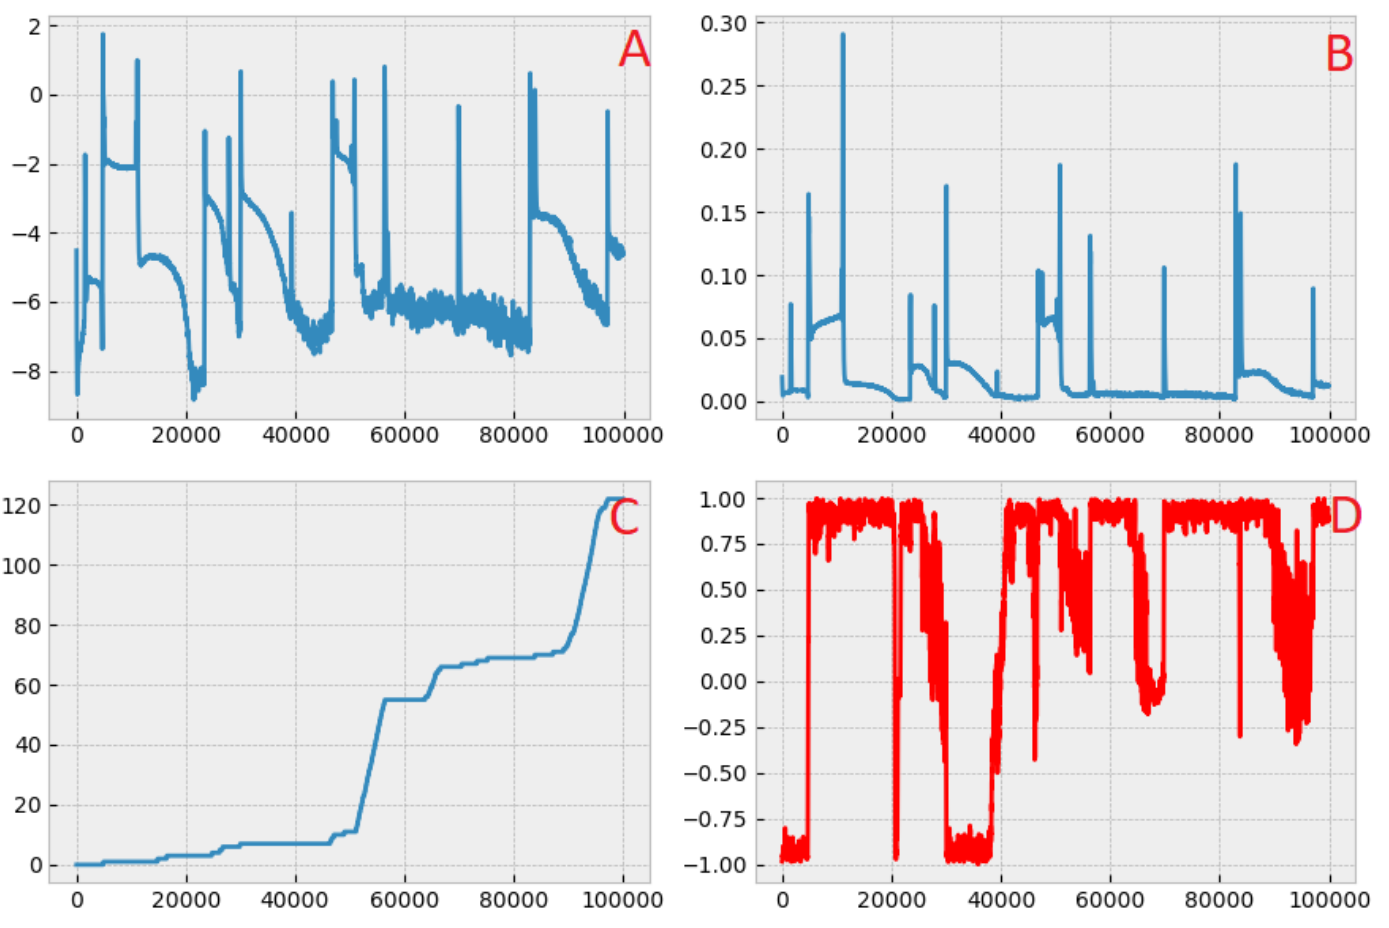
\includegraphics[width=0.5\paperwidth]{figure/fig10.PNG}\caption{\textbf{\emph{A)}}\emph{ shows the log of the training loss (moving
average with window 100), }\textbf{\emph{B}}\emph{) is the TD error,
}\textbf{\emph{C)}}\emph{ shows the cumulative reward, and }\textbf{\emph{D)}}\emph{
is the action chosen by the agent. On the 4 graphs, the x axis is
the number of training batches. There are 3 phases of good performance,
where the agent actually reaps many rewards (around steps 50000, 65000,
and 90000). These are followed by forgetting - the agent stops exploiting
the strategy that leads to high reward. Note that the total loss at
these times is not always decreasing, which is bewildering. It means
that the agent can learn without its loss visually decreasing. We
believe that a low loss should be strongly correlated with good performance
for the agent to be able to learn something. Minimizing the loss should
be a proxy for maximizing the cumulated reward. Note that most of
the time (graph D), the agent is just accelerating blindly, and it
is just when it stops doing so that it starts learning something useful
and obtaining rewards.}}
\par\end{centering}
\end{figure}

For a very long time, the agent just accelerates blindly, thus oscillating
between points A and B visible in Figure \ref{fig:Mountain-Car-Continuous.}.
Sometimes, it does the same but in the other direction. At some point,
it tries going backwards instead (it may be due to noise). After having
reached a far left position, it starts accelerating again, which allows
it to reach the flag at last. After having reached it once, it starts
exploiting the high reward path found many times in a row, until catastrophic
forgetting happens and the agent starts accelerating blindly again.
Over 100000 batches, there are several cycles of this phenomenon.
Obtaining a decent policy therefore requires to stop training at a
smart moment: when the agent reaps many rewards in a short time interval.
We observed the policies obtained at these smart moments to see whether
they looked sensible or not.

\begin{figure}[H]
\begin{centering}
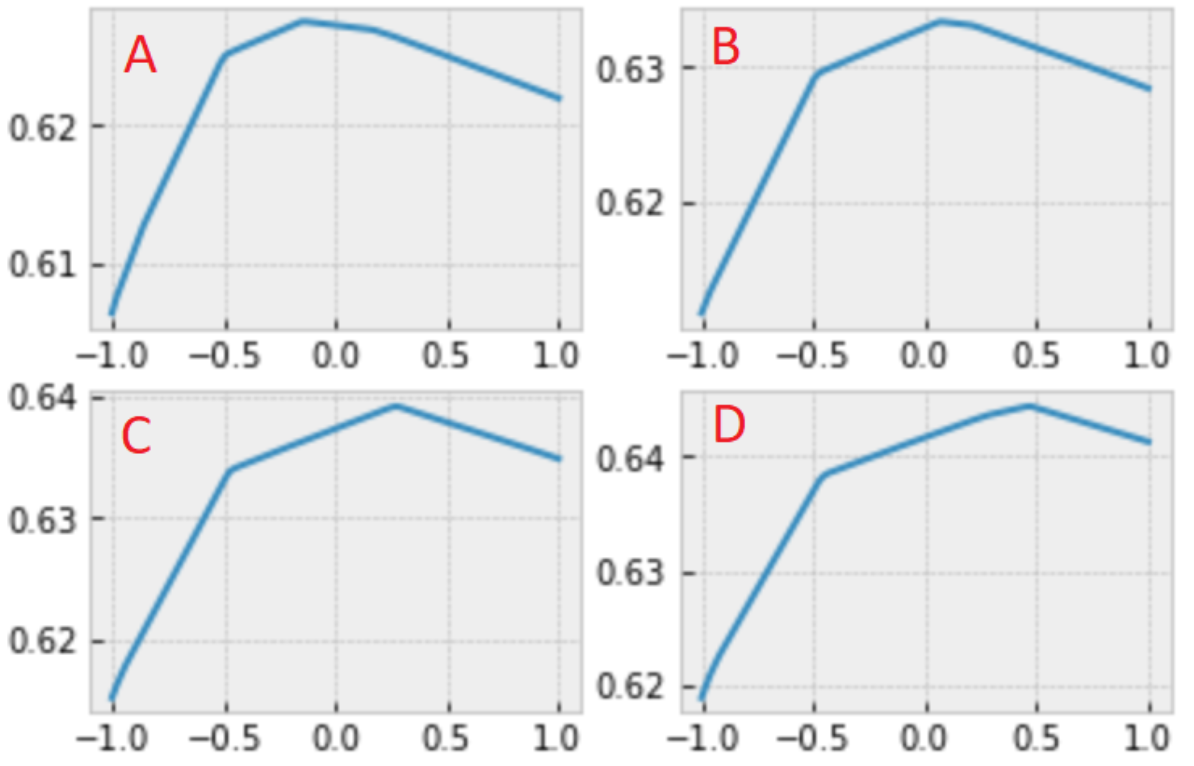
\includegraphics[width=0.5\paperwidth]{figure/fig11.PNG}
\par\end{centering}
\caption{output of a trained model with Tensorflow. On the four graphs, the
position is the same (0.2). The speed of the agent is different and
goes linearly from 0.01 to 0.04 between A and D. Note that the range
of possible positions goes from -1.2 to 0.6, and the speed from -0.07
to 0.07. What we observe is that if the agent is not fast enough at
this point, it prefers a negative acceleration to find itself in a
position where a positive acceleration will lead to the flag. It is
sensible because keeping on accelerating may be useless because of
gravity. Conversely, if its speed is high enough, it tries to continue
accelerating to reach the flag.}

\end{figure}

\begin{figure}[H]
\begin{centering}
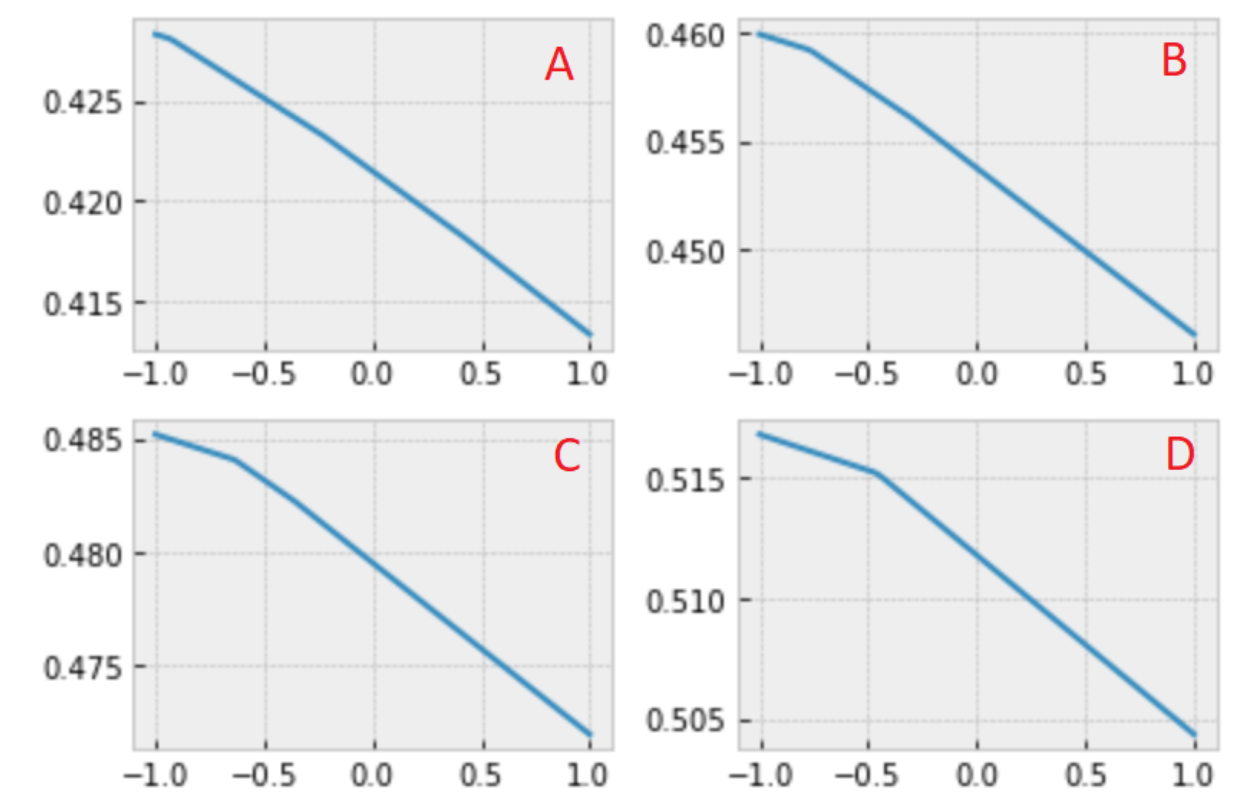
\includegraphics[width=0.5\paperwidth]{figure/fig12.PNG}
\par\end{centering}
\caption{output of a trained model with the Tensorflow implementation. On the
four graphs, the position is the same (-0.5, which is near to the
initial position). The speed of the agent is changes and is -0.07
in A, -0.02 in B, 0.02 in C, and 0.07 in D. Note that the range of
possible positions goes from -1.2 to 0.6, and the speed from -0.07
to 0.07. Here the policy does not make sense at all. Whatever the
speed is, the agent tries to go backward, while its speed should let
it reaches the flag for D at least, and maybe also for C. In A and
B it makes sense to go backward.}
\end{figure}

\subsection{Evaluation}

Evaluating our policies in the sepsis case requires careful consideration,
as we deal with some important challenges: firstly, the policy that
generated the data available in the MIMIC dataset is unknown, and
hard to estimate correctly, as it needs to approximate the behavior
of different clinicians, with different decision making processes,
in a complex state-space. Secondly, we are dealing with continuous
state and action spaces, and as such the computation of importance
weights has to be done with integrals instead of the classical sum.
Thirdly, our histories are limited in step size (some going as low
as 4 steps. DR and WDR estimators where implemented in the following
way:

\paragraph{Clinician policy estimation: }

To obtain a reliable clinician policy estimation, we first studied
the case stemming from a discretization of states and actions. Following
previous work by Komorowski et al. (2016), we solved an MDP on the
sepsis case with 750 discrete states and 25 discrete actions over
intravenous fluid and vasopressor dosage. We obtained a Q table that
will be denominated \emph{Q clinician, }from which it is possible
to obtain the policy for each state s by computing $argmax_{a}Q_{clinician}(s,a)$.
The policy obtained here is discrete, which is incompatible with our
continuous approach. To be able to make use of this policy as our
$\pi_{behavior}$, we tried multiple approaches. 
\begin{itemize}
\item We transformed the policy to a continuous one by thinking of it as
a continuous Dirac's delta on the center of the bin corresponding
to the action of maximum Q value. 
\item The value of $\pi_{behavior}$ for a particular state and action was
estimated as the number of actions in the dataset belonging to that
bin over the total number of actions. This corresponds to a discretization
of the states and actions that enter the pi\_behavior function, and
was done with a KD-Tree, a structure that allows fast lookups of nearest-neighbors.
\item We generated a continuous approximation over the state and action
space by overlapping gaussians centered on each centroid of the original
clustering, and with $\sigma=d_{sa}/4$, $d_{sa}$ being the mean
distance between each 52-dimensional centroid. The gaussians were
scaled by the value of the discrete $Q_{clinician}$ for each centroid.
\end{itemize}
In Doina et al., 2000, it is mentioned that the behavior policy must
be \emph{soft}, meaning that it must have a non-zero probability of
selecting every action in each state. This is arguably the reason
why, as can be seen in the results section, our first approach performed
erratically.

\paragraph{Evaluation policy: }

The output of the ICNN gives us the value of Q for a particular continuous
state and action. To approximate the value of $\pi_{e}$, we then
compute:
\[
\pi_{e}(s,a)=\frac{Q(s,a)-min_{a}Q(s,a)}{\int_{a}Q(s,a)-min_{a}Q(s,a)da}
\]

Where the division by the integral is meant to normalize $Q(s,a)-min_{a}Q(s,a)$,
and thus approximate a probability distribution over actions, necessary
characteristic of stochastic policies.

\paragraph{Estimations of Q and V:}

The WDR requires an estimation of the Q and V functions to compute
the Approximate Model part of its equation. In our case, the ICNN
is directly yielding an estimation of Q, $\hat{q}_{icnn}$. As or
$\hat{v}$, we calculate the following:
\[
\hat{v}(s)=\int\pi_{e}(s,a)\hat{q}_{icnn}(s,a)da
\]

This respects the definition of the value function in the continuous
case, but provides an estimation that depends on the accuracy of the
ICNN. 

\paragraph{Implementation details:}

The WDR calculation was performed with the course's provided function,
with minor alterations to facilitate the handling of continuous functions
instead of tables. The minimization of the Q function was performed
so as to leverage the concavity of the network: given that property,
the minimum of the Q function lies at one of the 4 corners of the
square action space. The minimizing function was then optimized so
as to only compute those four values and return the minimum. The arg-maximization
of the network is also facilitated by the ICNN properties. We applied
SGD to converge towards the maximum of the net by tweaking PyTorch
properties on the input parameters corresponding to the actions. 

One important aspect to remark is that the integral computation can
be very slow. It involves computing the Riemann sum, a numerical approximation
of the integral on the square corresponding to the action space. For
that computation, it is required to do forward passes over the icnn
for each point of a predefined grid over the action space. We worked
on a 20x20 grid, which translates to 400 forward passes each time
an integral has to be calculated. This proved to be extremely costly,
so another approach was implemented: a simple fully connected neural
network for integral prediction. The idea was to train this network
on integrals computed by the trained version of the ICNN previous
to the evaluation step, and then use the integral-predicting network
instead of calculating the Riemann sum. The results are shown in the
corresponding section.

This evaluation setup was tested on the Sepsis case as well as the
MountainCarContinuous environment. In the latter, we used the vanilla
DQN available as solution on the OpenAI Gym as our $\pi_{b}$ and
history generator: we applied the same transformations as for the
$\pi_{e}$ in the ICNN case, generated 300 histories of 30 to 900
episodes each, and calculated DR and WDR estimators with that dataset.

Evaluating the policies proved to be time consumming, but the results
are interesting. We applied the methods described in the previous
section to the Sepsis PyTorch implementation, MountainCar Pytorch
and MountainCar Tensorflow. We compared the obtined values to baselines
values that we believe to be accurate: for the sepsis case, we look
at the estimated value computed from Matthieu's DDQN implementation.
The results were as follows:
\begin{center}
\begin{tabular}{|c|c|c|c|}
\hline 
 & Sepsis & MountainCar PyTorch & MountainCar Tensorflow\tabularnewline
\hline 
\hline 
DR &  &  & -1.45\tabularnewline
\hline 
WDR - Dirac &  &  & \tabularnewline
\hline 
WDR - Gaussians &  &  & -1\tabularnewline
\hline 
WDR - integral prediction &  & NA & NA\tabularnewline
\hline 
Baseline &  &  & \tabularnewline
\hline 
\end{tabular}
\par\end{center}

It is interesting to see that the 

\section{Conclusion }

Unfortunately, we were unable to achieve positive results in the task
we undertook. While it seems sound theoretically, deep ICNNs proved
quite difficult to correctly build and train. These ideas need more
exploration. On the VAE side, more time should be devoted to exploring
the variational recurrent autoencoders \cite{fabius2014variational,krishnan2017structured}. 

\section{References}

\bibliographystyle{plain}
\bibliography{BibTex_final_project}

\end{document}
